
\section{Indirekter digitaler Reglerentwurf}

\subsection{Approximationen für Diskretisierung}{226}

\begin{minipage}[c]{0.48\columnwidth}
    Ein kontinuierlicher Regler (hier I-Regler) weist folgendes Verhalten auf:
\end{minipage}
\hfill
\begin{minipage}[c]{0.48\columnwidth}
    $$ u(t) = K_R \cdot \int\limits_0^t e(\tau) \, \diff \tau $$
\end{minipage}


Der entsprechende zeitdiskrete Regler kann \textbf{nicht exakt} gebildet werden, da $e(t)$ nur zu diskreten Zeitpunkten $e(kT)$ bekannt ist.
Geht man davon aus, dass $e(t)$ \textbf{nicht start ändert} (\textrightarrow\ geeignete Wahl der Abtastzeit $T$), dann kann $u(k)$
folgendermassen approximiert werden:

\vspace{-0.2cm}

$$ u(k) = K_R \cdot \int\limits_0^{kT} e(\tau) \, \diff \tau
    = \underbrace{K_R \cdot \int\limits_0^{kT- T} e(\tau) \, \diff \tau}_{u(k-1)} 
    + \underbrace{K_R \cdot \int\limits_{kT-T}^{kT} e(\tau) \, \diff \tau}_{\approx A} $$


\subsubsection{Approximationen der Fläche $\bm{A}$}

Die Fläche $A$ kann auf mehrere Arten approximiert werden:


\begin{minipage}[c]{0.35\columnwidth}
    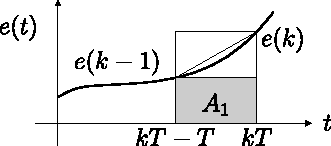
\includegraphics[width=\columnwidth, align=t]{images/dig_reg_approximation_integration.pdf}
\end{minipage}
\hfill
\begin{minipage}[c]{0.64\columnwidth}
    \resizebox{\columnwidth}{!}
    {
        \renewcommand{\arraystretch}{1.3}
        \begin{tabular}{ll@{}}
            Rechteckregel vorwärts (Euler)      & $A = T \cdot e(k-1)$                      \\
            Rechteckregel rückwärts             & $A = T \cdot e(k)$                        \\
            \textbf{Trapezregel (Tustin)}       & $A = T \cdot \dfrac{e(k-1) + e(k)}{2} $ 
        \end{tabular}
        \renewcommand{\arraystretch}{1}
    }
\end{minipage}

\vspace{0.2cm}
\textbf{Hinweis:} Für die Diskretisierung von Reglern wird die \textbf{Trapez-Approximation} verwendet, da diese am genausten ist.


\subsection{Vorgehen: Diskretisierung eines Reglers}{226-228}

Die Ordnung des Reglers bleibt bei der Diskretisierung erhalten.

$$ G_R(s) = \frac{U(s)}{E(s)} = \frac{b_m s^m + b_{m-1} s^{m-1} + \ldots + b_1 s + b_0}{s^n + a_{n-1} s^{n-1} + \ldots + a_1 s + a_0} \quad (m \leq n) $$
$$ \overline{G}_R(z) = \frac{U(z)}{E(z)} = \frac{\overline{b}_m z^m + \overline{b}_{m-1} z^{m-1} + \ldots + \overline{b}_1 z + \overline{b}_0}{z^n + \overline{a}_{n-1} z^{n-1} + \ldots + \overline{a}_1 z + \overline{a}_0} $$

\begin{enumerate}
    \item UTF des Reglers $G_R(s)$ bestimmen
    \item Wahl der Abtastzeit $T$ und Diskretisierungsmethode \textrightarrow\ typischerweise \textbf{Tustin}
    \item Transformation zu $\overline{G}_R(z)$  durch Substitution aller Variablen $s$ in $G_R(s)$ mit gewünschter Approximation \textrightarrow\ siehe Abschnitt \ref{Approximationsmethoden -- Substitutionsterme}
    \item Falls nötig: Doppelbrüche in $\overline{G}_R(z)$ eliminieren und $T$ numerisch einsetzen
    \item $\overline{G}_R(z)$ 'separieren' und ausmultiplizieren \\
        $\overline{b}_m z^m \cdot E(z) + \ldots + \overline{b}_1 z \cdot E(z) + \overline{b}_0 \cdot E(z) = z^n \cdot U(z) + \ldots + \overline{a}_1 z \cdot U(z) + \overline{a}_0 \cdot U(z)$
    \item Umformen in Differenzengleichung \\
        $\overline{b}_m \cdot e(k+m)  + \ldots + \overline{b}_1 \cdot e(k+1) + \overline{b}_0 \cdot e(k) = u(k+n) + \ldots + \overline{a}_1 \cdot u(k+1) + \overline{a}_0 \cdot u(k)$
    \item Resultierende zeitinvariante Gleichung $u(k)$ auflösen und bei Bedarf um $n$ Zeitschritte verschieben
\end{enumerate}



\subsubsection{Substitutionsterme z-Transformation}{227}
\label{Approximationsmethoden -- Substitutionsterme}

\begin{ctabular}{lcc}
    \toprule
    \textbf{Methode}                & \textbf{Substitution von} $\bm{s}$                & \textbf{Substitution von} $\bm{z}$    \\
    \midrule
    Rechteckregel vorwärts (Euler)  & $s = \frac{z - 1}{T}$                             & $z = 1 + sT$                          \\
    \midrule
    Rechteckregel rückwärts         & $s = \frac{1}{T} \cdot \frac{z - 1}{z}$           & $z = \frac{1}{1 - sT}$                \\
    \midrule
    \textbf{Tustin}                 & $\bm{s = \frac{2}{T} \cdot \frac{z - 1}{z + 1}}$  & $z = \frac{2 + sT}{2 - sT}$           \\
    \bottomrule
\end{ctabular}


% \begin{center}
%     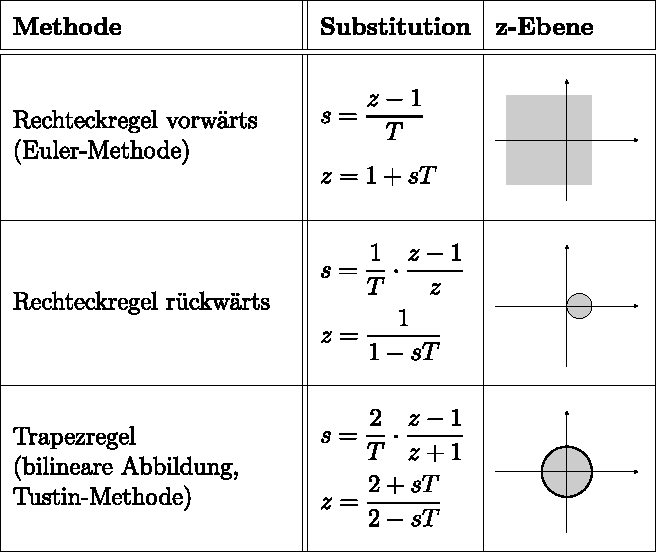
\includegraphics[width=0.8\columnwidth, align=t]{images/dig_reg_substitution_z_trafo.pdf}
% \end{center}


\example{Lead-Regler diskretisieren}

Gegeben sei die Übertragungsfunktion $G_R(s)$ eines \textbf{kontinuierlichen} Reglers.
Daraus soll die zu implementierende \textbf{Differenzengleichung} ermittelt werden. 

\vspace{-0.2cm}

\begin{ctabular}{lcl}
    \tabitem Diskretisierungsmethode: \textbf{Tustin}   &   & \tabitem Abtastzeit: $T = 0.1 \, \second$
\end{ctabular}

\vspace{-0.3cm}

$$ \bm{1.} \quad G_R(s) = 4 \cdot \frac{s+1}{s+5} \quad {\textrightarrow\ } \bm{2.} $$
$$ \overline{G}_{R}(z) \overset{\bm{3.}}{=} 4 \cdot \frac{1 + \frac{2}{T} \frac{z-1}{z+1}}{5 + \frac{2}{T} \frac{z-1}{z+1}} 
    \overset{\bm{4.}}{=} 4 \cdot \frac{T (z+1) + 2 (z-1)}{5 T (z+1) + 2 (z-1)} = \frac{3.36 z - 3.04}{z - 0.6} = \frac{U(z)}{E(z)} $$
$$ \bm{5.} \quad z \cdot U(z) - 0.6 \cdot U(z) = 3.36 z \cdot E(z) - 3.04 \cdot E(z) $$
$$ \bm{6.} \quad u(k+1) - 0.6 \cdot u(k) = 3.36 \cdot e(k+1) - 3.04 \cdot e(k) \qquad \big| \text{-1 Zeitschritt} $$
$$ \bm{7.} \quad u(k) = 0.6 \cdot u(k-1) + 3.36 \cdot e(k) - 3.04 \cdot e(k-1) $$


\subsection{Empirische Einstellregeln für digitale PID-Regler}

Für eine Strecke mit Totzeit $G_S(s)$ wird ein \textbf{zeitkontinuierlicher} PID-Regler mit UTF $G_R(s)$ entworfen.
Dieser kann mit den empirischen Einstellregeln von Ziegler-Nichols parametrisiert werden.

\vspace{-0.2cm}

$$ 
    G_S(s) = \frac{K_S}{s T_g + 1} \cdot e^{- s T_u} \qquad \qquad
    G_R(s) = K_R \left( 1 + \frac{1}{s T_N} + s T_V \right)
$$

Wird der \textbf{PID-Regler diskretisiert}, so kann er nach den Regeln von \textbf{Takahashi, Chan und Auslander} empirisch eingestellt werden (siehe Abschnitt \ref{Einstellregeln nach Takahashi, Chan und Auslander}).


\subsubsection{Einstellregeln nach Takahashi, Chan und Auslander}{230}
\label{Einstellregeln nach Takahashi, Chan und Auslander}

\textbf{Voraussetzung: } $\bm{T \leq 2 T_u}$

\begin{ctabular}{l c c c}
    \toprule
    \textbf{Regler}     & $\bm{K_R}$                                        & $\bm{T_N}$                                & $\bm{T_V}$                    \\
    \midrule
    P-Regler            & $\frac{T_g}{K_S (T_u + T)}$                       & $-$                                       & $-$                           \\
    \midrule
    PI-Regler           & $0.9 \cdot \frac{T_g}{K_S (T_u + \frac{T}{2})}$   & $3.33 \left( T_u + \frac{T}{2} \right)$   & $-$                           \\
    \midrule
    PID-Regler          & $1.2 \cdot \frac{T_g}{K_S (T_u + T)}$             & $ \left( T_u + \frac{T}{2} \right)$       & $0.5 \left( T_u + T \right)$  \\
    \bottomrule
\end{ctabular}

\textbf{Hinweis:} Für eine Abtastzeit von $T=0$ entspricht obige Tabelle der zeitkontinuerlichen Ziegler-Nichols Approximation.

